% 10-25 (user): the two forms of the document side by side -- same process outputs and feedback, different estimates and expected a-hat.
%   Wording as TIE 2025 (process outputs, estimator, motion control law); notation as 1025_wall_angle_estimator.tex.
\documentclass[border=8pt]{standalone}
\usepackage{amsmath,amssymb,bm,upgreek}
\usepackage{tikz}
\usetikzlibrary{arrows.meta,positioning,calc}
\newcommand{\bth}{\bm{\uptheta}}
\newcommand{\T}{T}
\begin{document}
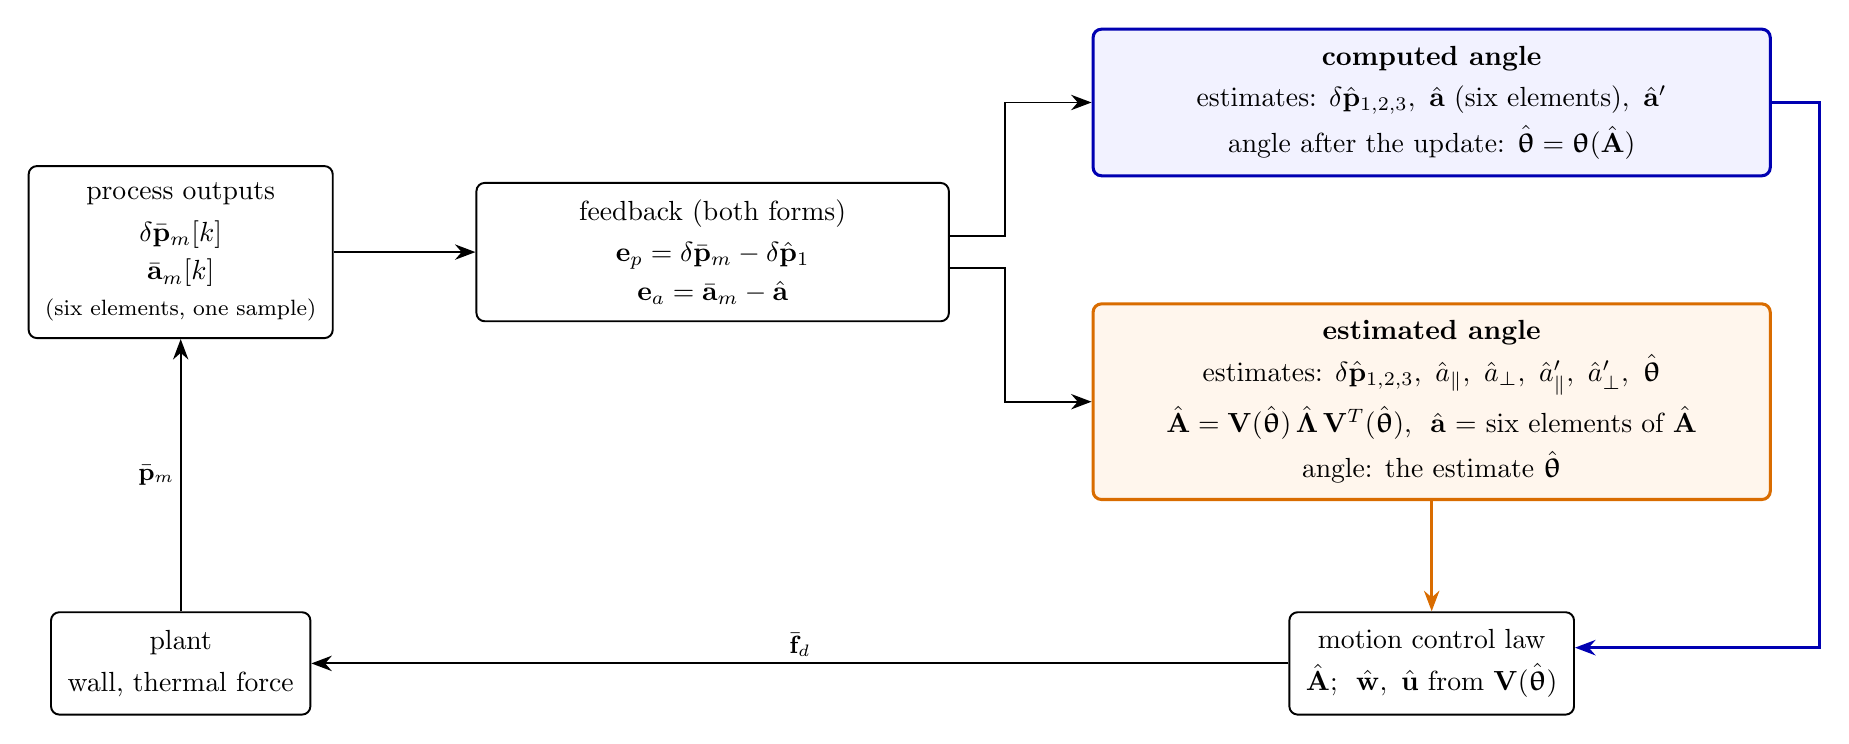
\begin{tikzpicture}[font=\normalsize, >={Stealth[length=2.6mm]}, line width=0.7pt,
  box/.style={draw, rounded corners=3pt, minimum height=13mm, align=center, fill=white, inner sep=6pt},
  cmp/.style={box, draw=blue!70!black, line width=1.1pt, fill=blue!5, minimum width=86mm},
  est/.style={box, draw=orange!85!black, line width=1.1pt, fill=orange!7, minimum width=86mm},
  lab/.style={font=\small, inner sep=2pt}]
\node[box] (out) {process outputs\\[3pt] $\delta\bar{\mathbf p}_m[k]$\\[2pt] $\bar{\mathbf a}_m[k]$\\[1pt] {\footnotesize (six elements, one sample)}};
\node[box, right=18mm of out, minimum width=60mm] (fb) {feedback (both forms)\\[3pt]
  $\mathbf e_p = \delta\bar{\mathbf p}_m - \delta\hat{\mathbf p}_1$\\[2pt] $\mathbf e_a = \bar{\mathbf a}_m - \hat{\mathbf a}$};
\node[cmp, right=18mm of fb, yshift=19mm] (c) {\textbf{computed angle}\\[3pt]
  estimates: $\delta\hat{\mathbf p}_{1,2,3},\ \hat{\mathbf a}\ (\text{six elements}),\ \hat{\mathbf a}'$\\[3pt]
  angle after the update: $\hat\bth = \bth(\hat{\mathbf A})$};
\node[est, right=18mm of fb, yshift=-19mm] (e) {\textbf{estimated angle}\\[3pt]
  estimates: $\delta\hat{\mathbf p}_{1,2,3},\ \hat a_\parallel,\ \hat a_\perp,\ \hat a'_\parallel,\ \hat a'_\perp,\ \hat\bth$\\[3pt]
  $\hat{\mathbf A} = \mathbf V(\hat\bth)\,\hat{\bm\Lambda}\,\mathbf V^{\T}(\hat\bth)$, \ $\hat{\mathbf a}$ = six elements of $\hat{\mathbf A}$\\[3pt]
  angle: the estimate $\hat\bth$};
\node[box, below=14mm of e] (cl) {motion control law\\[3pt] $\hat{\mathbf A}$; \ $\hat{\mathbf w},\ \hat{\mathbf u}$ from $\mathbf V(\hat\bth)$};
\node[box] at (cl -| out) (pl) {plant\\[3pt] wall, thermal force};
\draw[->] (out) -- (fb);
\draw[->] (fb.east) ++(0,2mm) -- ++(7mm,0) |- (c.west);
\draw[->] (fb.east) ++(0,-2mm) -- ++(7mm,0) |- (e.west);
\draw[->, blue!70!black, line width=1.1pt] (c.east) -- ++(6mm,0) |- ([yshift=2mm]cl.east);
\draw[->, orange!85!black, line width=1.1pt] (e.south) -- (cl.north);
\draw[->] (cl) -- node[lab, above] {$\bar{\mathbf f}_d$} (pl);
\draw[->] (pl) -- node[lab, left] {$\bar{\mathbf p}_m$} (out);
\end{tikzpicture}
\end{document}
